% Options for packages loaded elsewhere
\PassOptionsToPackage{unicode}{hyperref}
\PassOptionsToPackage{hyphens}{url}
%
\documentclass[
]{article}
\usepackage{lmodern}
\usepackage{amsmath}
\usepackage{ifxetex,ifluatex}
\ifnum 0\ifxetex 1\fi\ifluatex 1\fi=0 % if pdftex
  \usepackage[T1]{fontenc}
  \usepackage[utf8]{inputenc}
  \usepackage{textcomp} % provide euro and other symbols
  \usepackage{amssymb}
\else % if luatex or xetex
  \usepackage{unicode-math}
  \defaultfontfeatures{Scale=MatchLowercase}
  \defaultfontfeatures[\rmfamily]{Ligatures=TeX,Scale=1}
\fi
% Use upquote if available, for straight quotes in verbatim environments
\IfFileExists{upquote.sty}{\usepackage{upquote}}{}
\IfFileExists{microtype.sty}{% use microtype if available
  \usepackage[]{microtype}
  \UseMicrotypeSet[protrusion]{basicmath} % disable protrusion for tt fonts
}{}
\makeatletter
\@ifundefined{KOMAClassName}{% if non-KOMA class
  \IfFileExists{parskip.sty}{%
    \usepackage{parskip}
  }{% else
    \setlength{\parindent}{0pt}
    \setlength{\parskip}{6pt plus 2pt minus 1pt}}
}{% if KOMA class
  \KOMAoptions{parskip=half}}
\makeatother
\usepackage{xcolor}
\IfFileExists{xurl.sty}{\usepackage{xurl}}{} % add URL line breaks if available
\IfFileExists{bookmark.sty}{\usepackage{bookmark}}{\usepackage{hyperref}}
\hypersetup{
  pdftitle={The Grammar of Graphics- V2.0},
  pdfauthor={Arvind Venkatadri},
  hidelinks,
  pdfcreator={LaTeX via pandoc}}
\urlstyle{same} % disable monospaced font for URLs
\usepackage[margin=1in]{geometry}
\usepackage{color}
\usepackage{fancyvrb}
\newcommand{\VerbBar}{|}
\newcommand{\VERB}{\Verb[commandchars=\\\{\}]}
\DefineVerbatimEnvironment{Highlighting}{Verbatim}{commandchars=\\\{\}}
% Add ',fontsize=\small' for more characters per line
\usepackage{framed}
\definecolor{shadecolor}{RGB}{248,248,248}
\newenvironment{Shaded}{\begin{snugshade}}{\end{snugshade}}
\newcommand{\AlertTok}[1]{\textcolor[rgb]{0.94,0.16,0.16}{#1}}
\newcommand{\AnnotationTok}[1]{\textcolor[rgb]{0.56,0.35,0.01}{\textbf{\textit{#1}}}}
\newcommand{\AttributeTok}[1]{\textcolor[rgb]{0.77,0.63,0.00}{#1}}
\newcommand{\BaseNTok}[1]{\textcolor[rgb]{0.00,0.00,0.81}{#1}}
\newcommand{\BuiltInTok}[1]{#1}
\newcommand{\CharTok}[1]{\textcolor[rgb]{0.31,0.60,0.02}{#1}}
\newcommand{\CommentTok}[1]{\textcolor[rgb]{0.56,0.35,0.01}{\textit{#1}}}
\newcommand{\CommentVarTok}[1]{\textcolor[rgb]{0.56,0.35,0.01}{\textbf{\textit{#1}}}}
\newcommand{\ConstantTok}[1]{\textcolor[rgb]{0.00,0.00,0.00}{#1}}
\newcommand{\ControlFlowTok}[1]{\textcolor[rgb]{0.13,0.29,0.53}{\textbf{#1}}}
\newcommand{\DataTypeTok}[1]{\textcolor[rgb]{0.13,0.29,0.53}{#1}}
\newcommand{\DecValTok}[1]{\textcolor[rgb]{0.00,0.00,0.81}{#1}}
\newcommand{\DocumentationTok}[1]{\textcolor[rgb]{0.56,0.35,0.01}{\textbf{\textit{#1}}}}
\newcommand{\ErrorTok}[1]{\textcolor[rgb]{0.64,0.00,0.00}{\textbf{#1}}}
\newcommand{\ExtensionTok}[1]{#1}
\newcommand{\FloatTok}[1]{\textcolor[rgb]{0.00,0.00,0.81}{#1}}
\newcommand{\FunctionTok}[1]{\textcolor[rgb]{0.00,0.00,0.00}{#1}}
\newcommand{\ImportTok}[1]{#1}
\newcommand{\InformationTok}[1]{\textcolor[rgb]{0.56,0.35,0.01}{\textbf{\textit{#1}}}}
\newcommand{\KeywordTok}[1]{\textcolor[rgb]{0.13,0.29,0.53}{\textbf{#1}}}
\newcommand{\NormalTok}[1]{#1}
\newcommand{\OperatorTok}[1]{\textcolor[rgb]{0.81,0.36,0.00}{\textbf{#1}}}
\newcommand{\OtherTok}[1]{\textcolor[rgb]{0.56,0.35,0.01}{#1}}
\newcommand{\PreprocessorTok}[1]{\textcolor[rgb]{0.56,0.35,0.01}{\textit{#1}}}
\newcommand{\RegionMarkerTok}[1]{#1}
\newcommand{\SpecialCharTok}[1]{\textcolor[rgb]{0.00,0.00,0.00}{#1}}
\newcommand{\SpecialStringTok}[1]{\textcolor[rgb]{0.31,0.60,0.02}{#1}}
\newcommand{\StringTok}[1]{\textcolor[rgb]{0.31,0.60,0.02}{#1}}
\newcommand{\VariableTok}[1]{\textcolor[rgb]{0.00,0.00,0.00}{#1}}
\newcommand{\VerbatimStringTok}[1]{\textcolor[rgb]{0.31,0.60,0.02}{#1}}
\newcommand{\WarningTok}[1]{\textcolor[rgb]{0.56,0.35,0.01}{\textbf{\textit{#1}}}}
\usepackage{graphicx}
\makeatletter
\def\maxwidth{\ifdim\Gin@nat@width>\linewidth\linewidth\else\Gin@nat@width\fi}
\def\maxheight{\ifdim\Gin@nat@height>\textheight\textheight\else\Gin@nat@height\fi}
\makeatother
% Scale images if necessary, so that they will not overflow the page
% margins by default, and it is still possible to overwrite the defaults
% using explicit options in \includegraphics[width, height, ...]{}
\setkeys{Gin}{width=\maxwidth,height=\maxheight,keepaspectratio}
% Set default figure placement to htbp
\makeatletter
\def\fps@figure{htbp}
\makeatother
\setlength{\emergencystretch}{3em} % prevent overfull lines
\providecommand{\tightlist}{%
  \setlength{\itemsep}{0pt}\setlength{\parskip}{0pt}}
\setcounter{secnumdepth}{-\maxdimen} % remove section numbering
\ifluatex
  \usepackage{selnolig}  % disable illegal ligatures
\fi

\title{The Grammar of Graphics- V2.0}
\author{Arvind Venkatadri}
\date{02 Feb 2021}

\begin{document}
\maketitle

{
\setcounter{tocdepth}{2}
\tableofcontents
}
This RMarkdown document is derived from \emph{A Layered Grammar of
Graphics} by Hadley Wickham, which is on the Files folder.

I strongly encourage you to glance through the original article, when
you work more with this document.

Esp. IAIDP,VCSB and HCD people. Oh, and FILM people.

\hypertarget{a-teaser-from-john-snow}{%
\subsection{A Teaser from John Snow}\label{a-teaser-from-john-snow}}

\begin{Shaded}
\begin{Highlighting}[]
\FunctionTok{SnowMap}\NormalTok{(}\AttributeTok{polygons =} \ConstantTok{TRUE}\NormalTok{)}
\end{Highlighting}
\end{Shaded}

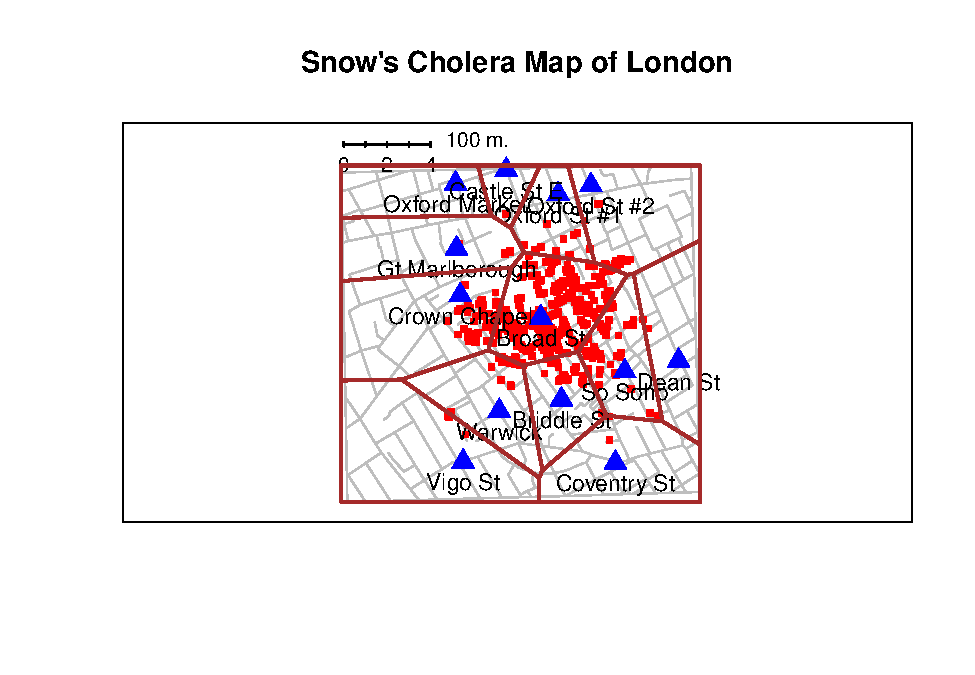
\includegraphics{Grammar-of-Graphics_files/figure-latex/teaser-1.pdf}

\begin{Shaded}
\begin{Highlighting}[]
\CommentTok{\# Write some comments on this code and what it seems to be creating}
\CommentTok{\# Are there "layers" in this visualization?}
\end{Highlighting}
\end{Shaded}

\hypertarget{components-of-the-layered-grammar-of-graphics}{%
\subsection{Components of the layered grammar of
graphics}\label{components-of-the-layered-grammar-of-graphics}}

\hypertarget{layer}{%
\subsubsection{Layer}\label{layer}}

\textbf{Layers} are used to create the objects on a plot. They are
defined by five basic parts:

\begin{enumerate}
\def\labelenumi{\arabic{enumi}.}
\tightlist
\item
  Data ( What dataset/spreadsheet am I using?)
\item
  Mapping ( What does each column do in my graph?)
\item
  Statistical transformation (stat) (Do I have calculate something
  first?)
\item
  Geometric object (geom) ( What shape, colour, size..do I want?)
\item
  Position adjustment (position) ( Where do I want it on the graph?)
\end{enumerate}

\hypertarget{tidy-data}{%
\paragraph{Tidy Data}\label{tidy-data}}

\begin{figure}
\centering
\includegraphics{https://raw.githubusercontent.com/allisonhorst/stats-illustrations/master/rstats-artwork/tidydata_1.jpg}
\caption{Tidy data}
\end{figure}

\hypertarget{kids-of-variables}{%
\paragraph{Kids of Variables}\label{kids-of-variables}}

\textbf{Kinds of Variable} are defined by the kind of questions they
answer to:

\begin{enumerate}
\def\labelenumi{\arabic{enumi}.}
\tightlist
\item
  What/Who/Where? -\textgreater{} Some kind of Name or Category
  (Remember Lars Gustaffson)
\item
  What Kind? How? -\textgreater{} Some kind ``Type''
\item
  How Many? How large? -\textgreater{} Some kind of Quantity
\end{enumerate}

\hypertarget{data-and-mapping}{%
\subsubsection{Data and mapping}\label{data-and-mapping}}

We will use ``real world'' data. Let's use the \texttt{penguins} dataset
in the \texttt{palmerpenguins} package.\footnote{Run \texttt{?penguins}
  in the console to get more information about this dataset.}

\begin{Shaded}
\begin{Highlighting}[]
\FunctionTok{head}\NormalTok{(penguins, }\AttributeTok{n =} \DecValTok{3}\NormalTok{)}
\end{Highlighting}
\end{Shaded}

\begin{verbatim}
## # A tibble: 3 x 8
##   species island bill_length_mm bill_depth_mm flipper_length_~ body_mass_g sex  
##   <fct>   <fct>           <dbl>         <dbl>            <int>       <int> <fct>
## 1 Adelie  Torge~           39.1          18.7              181        3750 male 
## 2 Adelie  Torge~           39.5          17.4              186        3800 fema~
## 3 Adelie  Torge~           40.3          18                195        3250 fema~
## # ... with 1 more variable: year <int>
\end{verbatim}

\begin{Shaded}
\begin{Highlighting}[]
\FunctionTok{tail}\NormalTok{(penguins)}
\end{Highlighting}
\end{Shaded}

\begin{verbatim}
## # A tibble: 6 x 8
##   species island bill_length_mm bill_depth_mm flipper_length_~ body_mass_g sex  
##   <fct>   <fct>           <dbl>         <dbl>            <int>       <int> <fct>
## 1 Chinst~ Dream            45.7          17                195        3650 fema~
## 2 Chinst~ Dream            55.8          19.8              207        4000 male 
## 3 Chinst~ Dream            43.5          18.1              202        3400 fema~
## 4 Chinst~ Dream            49.6          18.2              193        3775 male 
## 5 Chinst~ Dream            50.8          19                210        4100 male 
## 6 Chinst~ Dream            50.2          18.7              198        3775 fema~
## # ... with 1 more variable: year <int>
\end{verbatim}

\begin{Shaded}
\begin{Highlighting}[]
\FunctionTok{dim}\NormalTok{(penguins)}
\end{Highlighting}
\end{Shaded}

\begin{verbatim}
## [1] 344   8
\end{verbatim}

\begin{Shaded}
\begin{Highlighting}[]
\NormalTok{?penguins}
\end{Highlighting}
\end{Shaded}

\textbf{Aesthetic Mapping} defines how the variables are applied to the
plot. So if we were graphing information from \texttt{penguins}, we
might map a penguin's flipper\_length\_mm to the \(x\) position and
body\_mass\_g to the \(y\) position. We can map variables metaphorically
to other things: shape, colour, size, alpha(how dark?)\ldots.

For our running example,

\begin{Shaded}
\begin{Highlighting}[]
\NormalTok{penguins }\SpecialCharTok{\%\textgreater{}\%}
  \FunctionTok{select}\NormalTok{(bill\_length\_mm,body\_mass\_g) }\SpecialCharTok{\%\textgreater{}\%}
  \FunctionTok{rename}\NormalTok{(}\AttributeTok{x =}\NormalTok{ bill\_length\_mm,}
         \AttributeTok{y =}\NormalTok{ body\_mass\_g)}
\end{Highlighting}
\end{Shaded}

\begin{verbatim}
## # A tibble: 344 x 2
##        x     y
##    <dbl> <int>
##  1  39.1  3750
##  2  39.5  3800
##  3  40.3  3250
##  4  NA      NA
##  5  36.7  3450
##  6  39.3  3650
##  7  38.9  3625
##  8  39.2  4675
##  9  34.1  3475
## 10  42    4250
## # ... with 334 more rows
\end{verbatim}

\begin{Shaded}
\begin{Highlighting}[]
\NormalTok{penguins }\SpecialCharTok{\%\textgreater{}\%} 
  \FunctionTok{ggplot}\NormalTok{(}\AttributeTok{mapping =} \FunctionTok{aes}\NormalTok{(}\AttributeTok{x =}\NormalTok{ bill\_length\_mm, }\AttributeTok{y =}\NormalTok{ body\_mass\_g)) }\SpecialCharTok{+}
  \FunctionTok{geom\_point}\NormalTok{() }\SpecialCharTok{+} 
  \FunctionTok{geom\_smooth}\NormalTok{(}\AttributeTok{method =} \StringTok{"lm"}\NormalTok{, }\AttributeTok{se =} \ConstantTok{TRUE}\NormalTok{)}
\end{Highlighting}
\end{Shaded}

\begin{verbatim}
## `geom_smooth()` using formula 'y ~ x'
\end{verbatim}

\begin{verbatim}
## Warning: Removed 2 rows containing non-finite values (stat_smooth).
\end{verbatim}

\begin{verbatim}
## Warning: Removed 2 rows containing missing values (geom_point).
\end{verbatim}

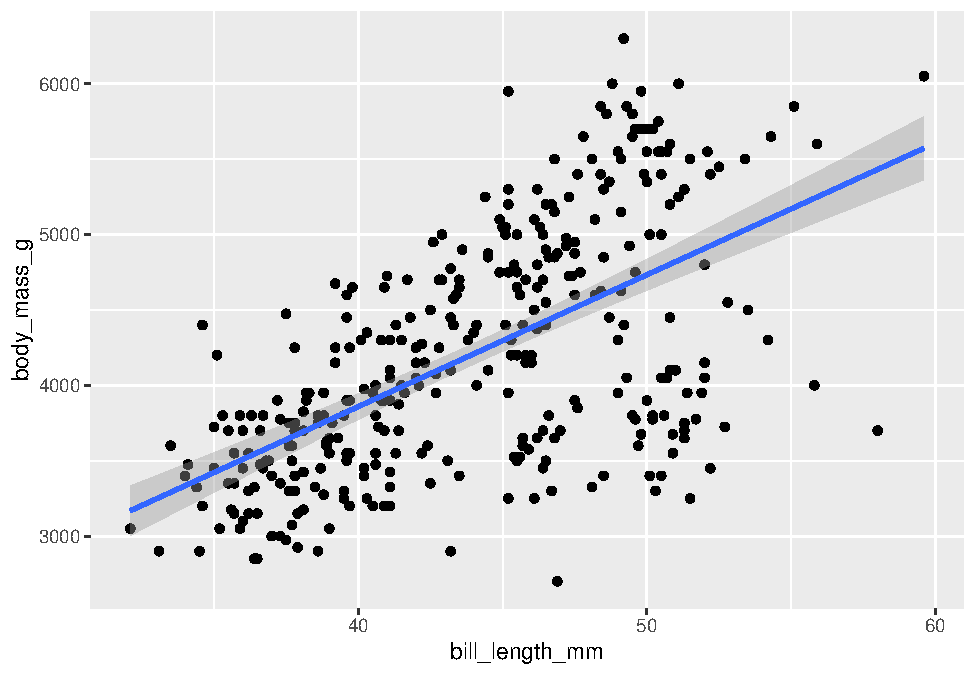
\includegraphics{Grammar-of-Graphics_files/figure-latex/mapping-1.pdf}

\hypertarget{statistical-transformation}{%
\subsection{Statistical
transformation}\label{statistical-transformation}}

A \textbf{statistical transformation} (\emph{stat}) transforms the data,
generally by summarizing the information. For instance, in a bar graph
you might summarize the data by graphing the total number of
observations within a set of categories.

A stat is a function that takes in a dataset as the input and returns a
dataset as the output; a stat can add new variables to the original
dataset, or create an entirely new dataset. So instead of graphing this
data in its raw form:

\begin{Shaded}
\begin{Highlighting}[]
\NormalTok{penguins }\SpecialCharTok{\%\textgreater{}\%}
  \FunctionTok{select}\NormalTok{(island)}
\end{Highlighting}
\end{Shaded}

\begin{verbatim}
## # A tibble: 344 x 1
##    island   
##    <fct>    
##  1 Torgersen
##  2 Torgersen
##  3 Torgersen
##  4 Torgersen
##  5 Torgersen
##  6 Torgersen
##  7 Torgersen
##  8 Torgersen
##  9 Torgersen
## 10 Torgersen
## # ... with 334 more rows
\end{verbatim}

You would transform it to:

\begin{Shaded}
\begin{Highlighting}[]
\NormalTok{penguins }\SpecialCharTok{\%\textgreater{}\%}
  \FunctionTok{count}\NormalTok{(island)}
\end{Highlighting}
\end{Shaded}

\begin{verbatim}
## # A tibble: 3 x 2
##   island        n
##   <fct>     <int>
## 1 Biscoe      168
## 2 Dream       124
## 3 Torgersen    52
\end{verbatim}

Sometimes you don't need to make a statistical transformation. For
example, in a scatterplot you use the raw values for the \(x\) and \(y\)
variables to map onto the graph. In these situations, the statistical
transformation is an \emph{identity} transformation - the stat simply
passes in the original dataset and exports the exact same dataset.

\hypertarget{geometric-objects}{%
\subsection{Geometric objects}\label{geometric-objects}}

\textbf{Geometric objects} (\emph{geoms}) control the type of plot you
create. Geoms are classified by their dimensionality:

\begin{itemize}
\tightlist
\item
  0 dimensions - point, text
\item
  1 dimension - path, line
\item
  2 dimensions - polygon, interval
\end{itemize}

Each geom can only display certain \textbf{aesthetics} or visual
attributes of the geom. For example, a point geom has position, color,
shape, and size aesthetics.

\begin{Shaded}
\begin{Highlighting}[]
\FunctionTok{ggplot}\NormalTok{(}\AttributeTok{data =}\NormalTok{ penguins, }
       \AttributeTok{mapping =} \FunctionTok{aes}\NormalTok{(}\AttributeTok{x =}\NormalTok{ bill\_length\_mm, }\CommentTok{\# x{-}position =\textgreater{} bill\_length\_mm}
                     \AttributeTok{y =}\NormalTok{ body\_mass\_g, }\CommentTok{\# y{-}position =\textgreater{} body\_mass\_g}
                     \AttributeTok{color =}\NormalTok{ island)) }\SpecialCharTok{+} \CommentTok{\# color =\textgreater{} Island as Metaphor}
  \FunctionTok{geom\_point}\NormalTok{() }\SpecialCharTok{+}
  \FunctionTok{ggtitle}\NormalTok{(}\StringTok{"A point geom with position and color aesthetics"}\NormalTok{)}
\end{Highlighting}
\end{Shaded}

\begin{verbatim}
## Warning: Removed 2 rows containing missing values (geom_point).
\end{verbatim}

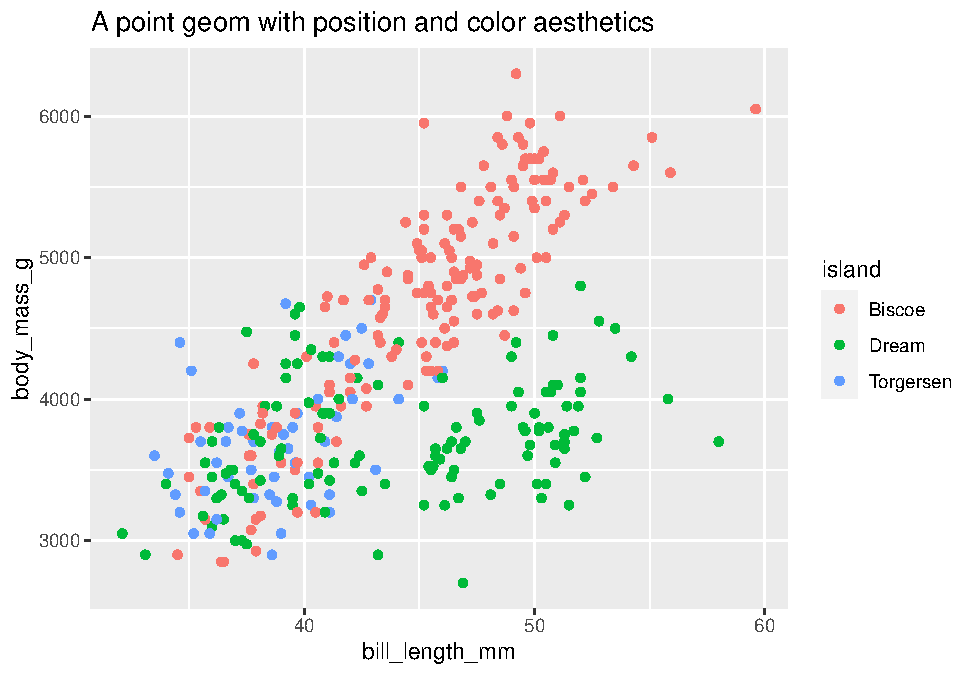
\includegraphics{Grammar-of-Graphics_files/figure-latex/geom_point_position_colour-1.pdf}

\begin{Shaded}
\begin{Highlighting}[]
\FunctionTok{ggplot}\NormalTok{(}\AttributeTok{data =}\NormalTok{ penguins, }
       \AttributeTok{mapping =} \FunctionTok{aes}\NormalTok{(}\AttributeTok{x =}\NormalTok{ bill\_length\_mm, }
                     \AttributeTok{y =}\NormalTok{ body\_mass\_g, }
                     \AttributeTok{color =}\NormalTok{ species, }
                     \AttributeTok{shape =}\NormalTok{ island)) }\SpecialCharTok{+}
  \FunctionTok{geom\_point}\NormalTok{() }\SpecialCharTok{+}
  \FunctionTok{ggtitle}\NormalTok{(}\StringTok{"A point geom with position and color and shape aesthetics"}\NormalTok{)}
\end{Highlighting}
\end{Shaded}

\begin{verbatim}
## Warning: Removed 2 rows containing missing values (geom_point).
\end{verbatim}

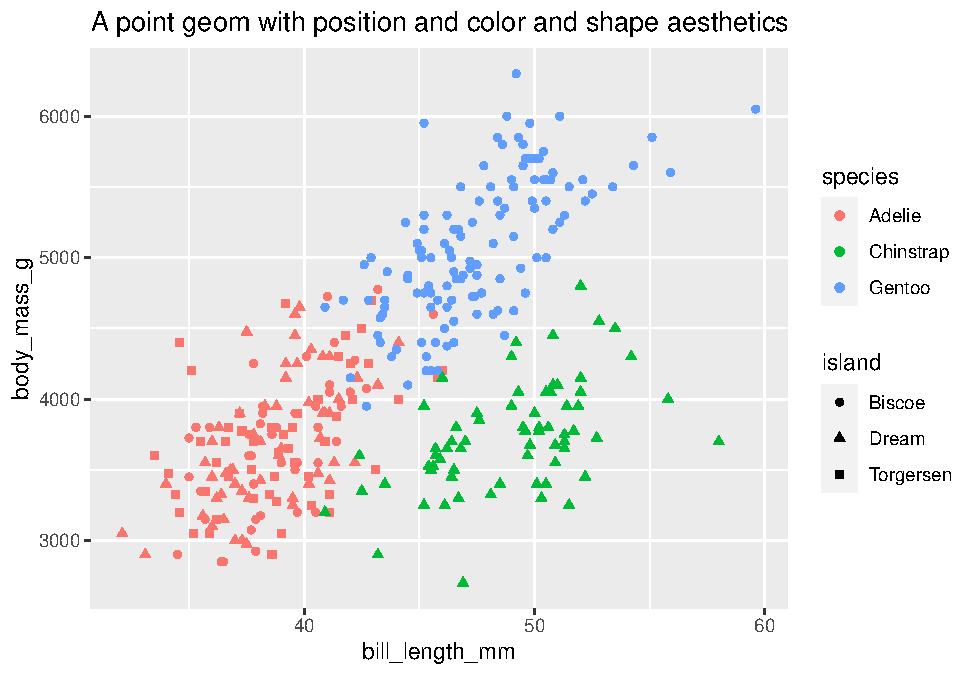
\includegraphics{Grammar-of-Graphics_files/figure-latex/geom_point_position_colour_shape-1.pdf}

\begin{itemize}
\tightlist
\item
  Position defines where each point is drawn on the plot
\item
  Color defines the color of each point. Here the color is determined by
  the class of the car (observation)
\end{itemize}

Whereas a bar geom has position, height, width, and fill color.

\begin{Shaded}
\begin{Highlighting}[]
\FunctionTok{ggplot}\NormalTok{(}\AttributeTok{data =}\NormalTok{ penguins, }
       \FunctionTok{aes}\NormalTok{(}\AttributeTok{x =}\NormalTok{ species)) }\SpecialCharTok{+} \CommentTok{\# x position =\textgreater{} ?}
  \CommentTok{\# No need to type "mapping"...}
  \FunctionTok{geom\_bar}\NormalTok{() }\SpecialCharTok{+} \CommentTok{\# Where does the height come from?}
  \FunctionTok{ggtitle}\NormalTok{(}\StringTok{"A bar geom with position and height aesthetics"}\NormalTok{)}
\end{Highlighting}
\end{Shaded}

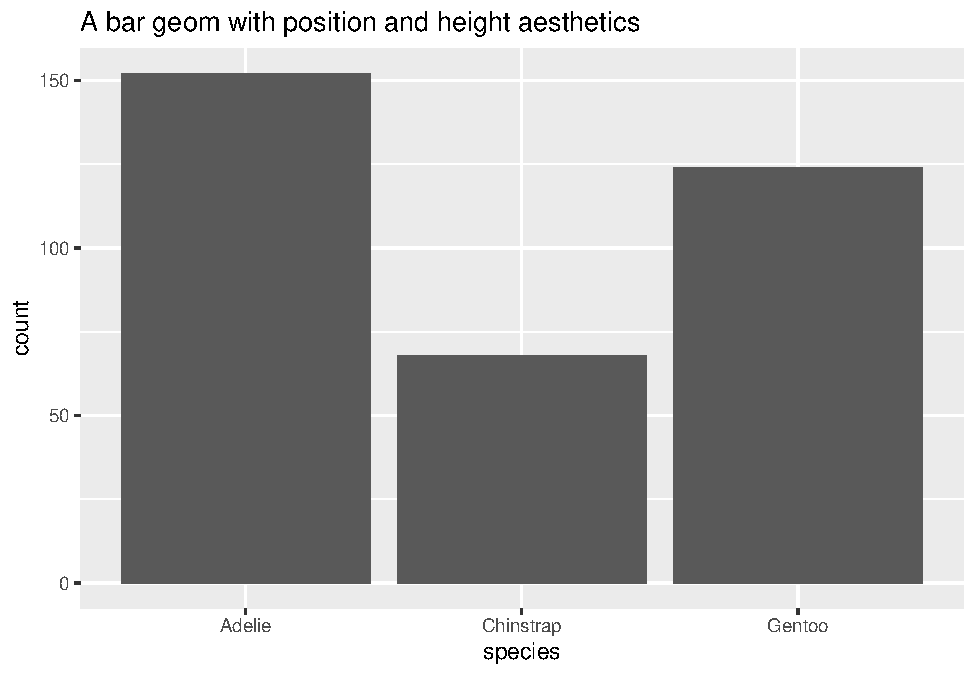
\includegraphics{Grammar-of-Graphics_files/figure-latex/geom_bar-1-1.pdf}

\begin{Shaded}
\begin{Highlighting}[]
\FunctionTok{ggplot}\NormalTok{(}\AttributeTok{data =}\NormalTok{ penguins, }\FunctionTok{aes}\NormalTok{(}\AttributeTok{x =}\NormalTok{ species)) }\SpecialCharTok{+}
  \FunctionTok{geom\_bar}\NormalTok{() }\SpecialCharTok{+}
  \FunctionTok{ggtitle}\NormalTok{(}\StringTok{"A bar geom with position and height aesthetics"}\NormalTok{)}
\end{Highlighting}
\end{Shaded}

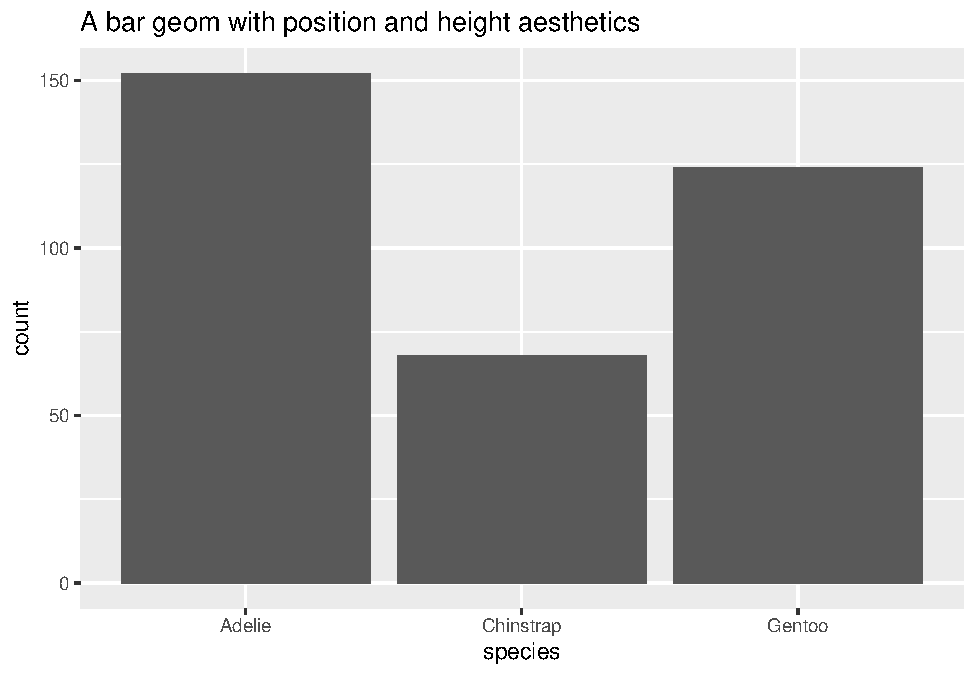
\includegraphics{Grammar-of-Graphics_files/figure-latex/geom_bar-2-1.pdf}

\begin{itemize}
\tightlist
\item
  Position determines the starting location (origin) of each bar
\item
  Height determines how tall to draw the bar. Here the height is based
  on the number of observations in the dataset for each possible number
  of cylinders.
\end{itemize}

\hypertarget{position-adjustment}{%
\subsection{Position adjustment}\label{position-adjustment}}

Sometimes with dense data we need to adjust the position of elements on
the plot, otherwise data points might obscure one another. Bar plots
frequently \textbf{stack} or \textbf{dodge} the bars to avoid overlap:

\begin{Shaded}
\begin{Highlighting}[]
\FunctionTok{count}\NormalTok{(}\AttributeTok{x =}\NormalTok{ penguins, species, island) }\SpecialCharTok{\%\textgreater{}\%}
  \FunctionTok{ggplot}\NormalTok{(}\AttributeTok{mapping =} \FunctionTok{aes}\NormalTok{(}\AttributeTok{x =}\NormalTok{ species, }\AttributeTok{y =}\NormalTok{ n, }\AttributeTok{fill =}\NormalTok{ island)) }\SpecialCharTok{+}
  \FunctionTok{geom\_bar}\NormalTok{(}\AttributeTok{stat =} \StringTok{"identity"}\NormalTok{) }\SpecialCharTok{+}
  \FunctionTok{ggtitle}\NormalTok{(}\AttributeTok{label =} \StringTok{"A stacked bar chart"}\NormalTok{)}
\end{Highlighting}
\end{Shaded}

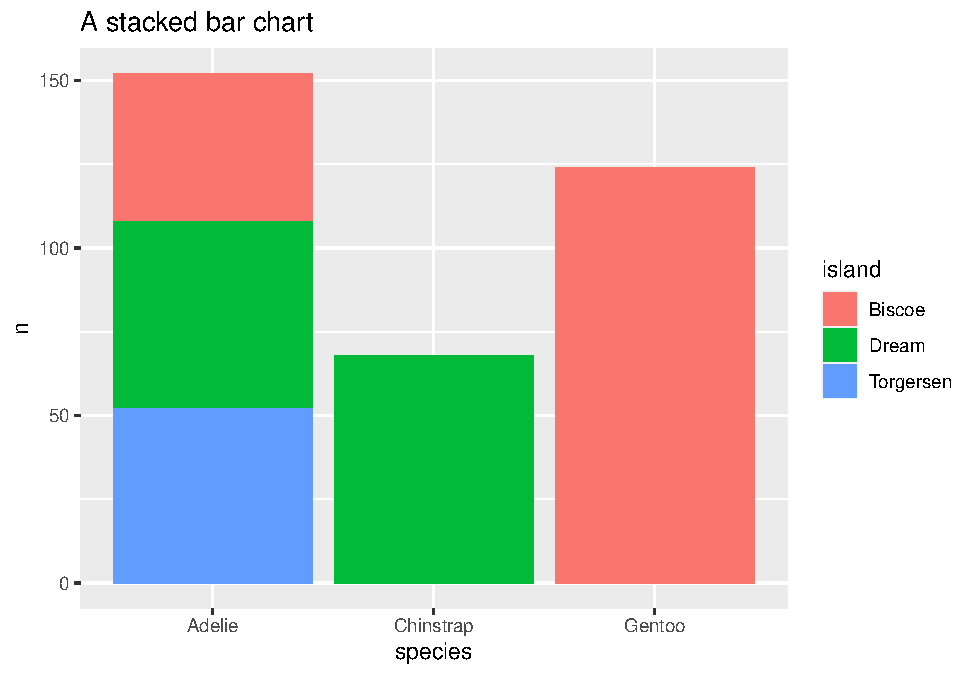
\includegraphics{Grammar-of-Graphics_files/figure-latex/geom_bar_position_stack_and_dodge-1.pdf}

\begin{Shaded}
\begin{Highlighting}[]
\FunctionTok{count}\NormalTok{(}\AttributeTok{x =}\NormalTok{ penguins, species, island) }\SpecialCharTok{\%\textgreater{}\%}
  \FunctionTok{ggplot}\NormalTok{(}\AttributeTok{mapping =} \FunctionTok{aes}\NormalTok{(}\AttributeTok{x =}\NormalTok{ species, }\AttributeTok{y =}\NormalTok{ n, }\AttributeTok{fill =}\NormalTok{ island)) }\SpecialCharTok{+}
  \FunctionTok{geom\_bar}\NormalTok{(}\AttributeTok{stat =} \StringTok{"identity"}\NormalTok{, }\AttributeTok{position =} \StringTok{"dodge"}\NormalTok{) }\SpecialCharTok{+}
  \FunctionTok{ggtitle}\NormalTok{(}\AttributeTok{label =} \StringTok{"A dodged bar chart"}\NormalTok{)}
\end{Highlighting}
\end{Shaded}

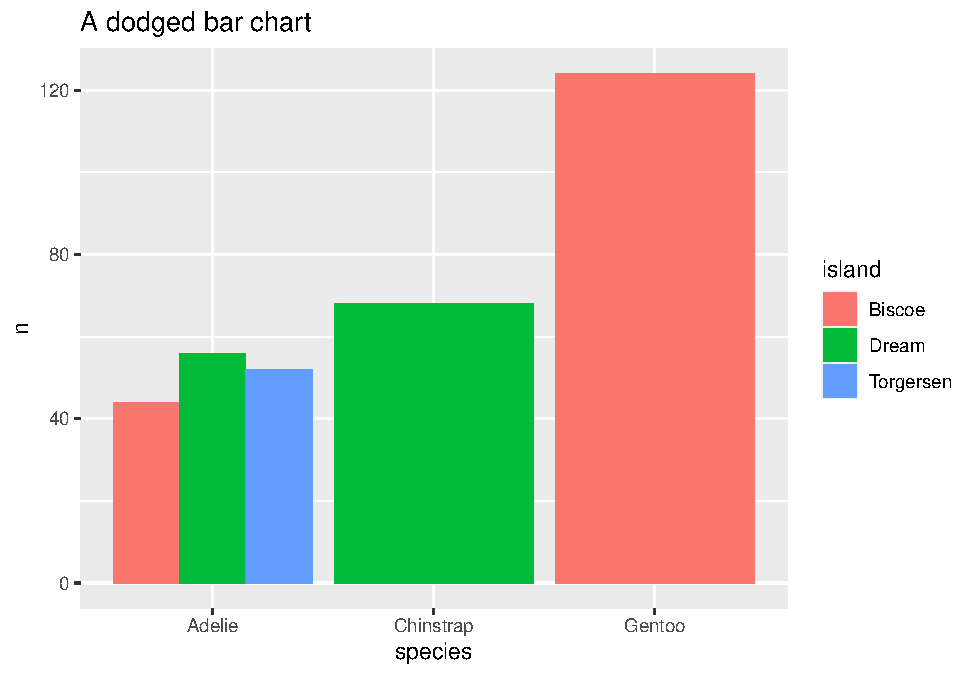
\includegraphics{Grammar-of-Graphics_files/figure-latex/geom_bar_position_stack_and_dodge-2.pdf}

\begin{Shaded}
\begin{Highlighting}[]
\NormalTok{penguins }\SpecialCharTok{\%\textgreater{}\%}
  \FunctionTok{ggplot}\NormalTok{(}\AttributeTok{mapping =} \FunctionTok{aes}\NormalTok{(}\AttributeTok{x =}\NormalTok{ species, }\AttributeTok{fill =}\NormalTok{ island)) }\SpecialCharTok{+}
  \FunctionTok{geom\_bar}\NormalTok{() }\SpecialCharTok{+}
  \FunctionTok{ggtitle}\NormalTok{(}\AttributeTok{label =} \StringTok{"A stacked bar chart"}\NormalTok{)}
\end{Highlighting}
\end{Shaded}

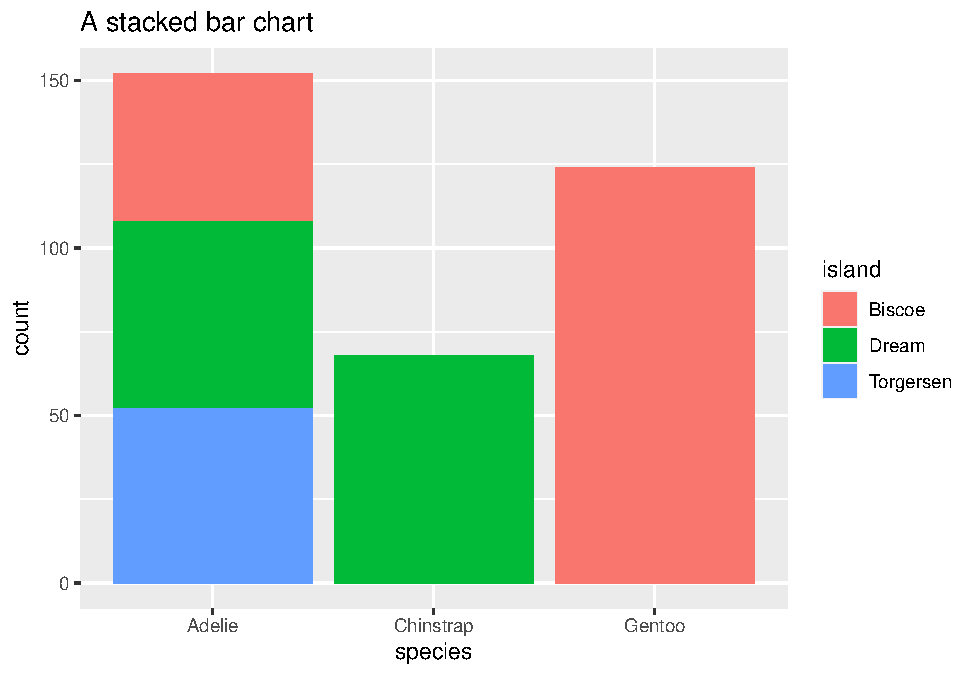
\includegraphics{Grammar-of-Graphics_files/figure-latex/unnamed-chunk-1-1.pdf}

\begin{Shaded}
\begin{Highlighting}[]
\NormalTok{penguins }\SpecialCharTok{\%\textgreater{}\%}
  \FunctionTok{ggplot}\NormalTok{(}\AttributeTok{mapping =} \FunctionTok{aes}\NormalTok{(}\AttributeTok{x =}\NormalTok{ species, }\AttributeTok{fill =}\NormalTok{ island)) }\SpecialCharTok{+}
  \FunctionTok{geom\_bar}\NormalTok{(}\AttributeTok{position =} \StringTok{"dodge"}\NormalTok{) }\SpecialCharTok{+}
  \FunctionTok{ggtitle}\NormalTok{(}\AttributeTok{label =} \StringTok{"A dodged bar chart"}\NormalTok{)}
\end{Highlighting}
\end{Shaded}

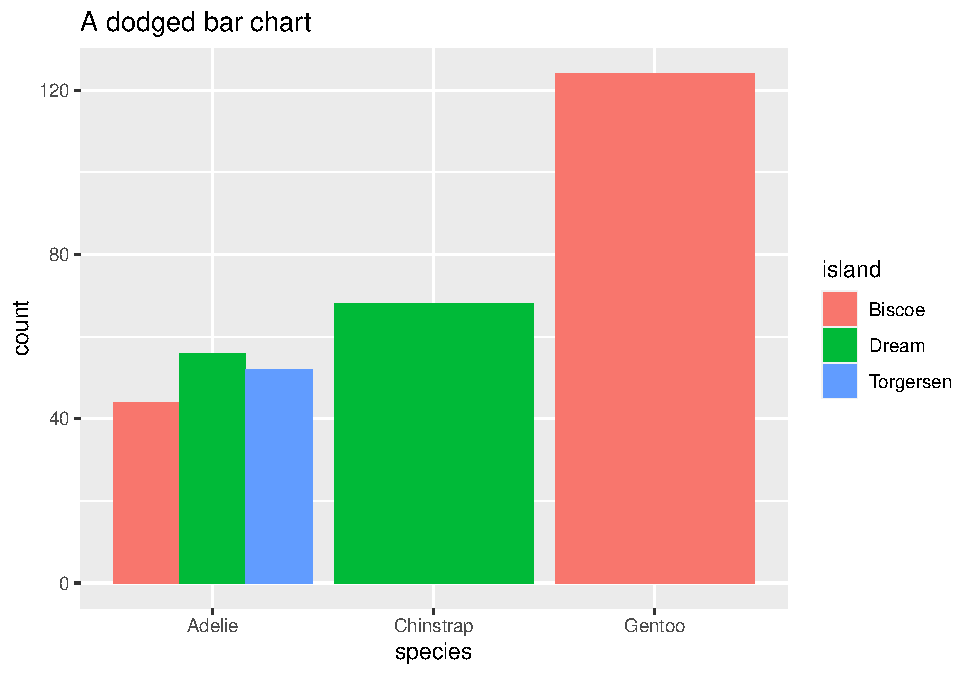
\includegraphics{Grammar-of-Graphics_files/figure-latex/unnamed-chunk-1-2.pdf}

Sometimes scatterplots with few unique \(x\) and \(y\) values are
\textbf{jittered} (random noise is added) to reduce overplotting.

\begin{Shaded}
\begin{Highlighting}[]
\FunctionTok{ggplot}\NormalTok{(}\AttributeTok{data =}\NormalTok{ penguins, }\AttributeTok{mapping =} \FunctionTok{aes}\NormalTok{(}\AttributeTok{x =}\NormalTok{ species, }\AttributeTok{y =}\NormalTok{ body\_mass\_g)) }\SpecialCharTok{+}
  \FunctionTok{geom\_point}\NormalTok{() }\SpecialCharTok{+}
  \FunctionTok{ggtitle}\NormalTok{(}\StringTok{"A point geom with obscured data points"}\NormalTok{)}
\end{Highlighting}
\end{Shaded}

\begin{verbatim}
## Warning: Removed 2 rows containing missing values (geom_point).
\end{verbatim}

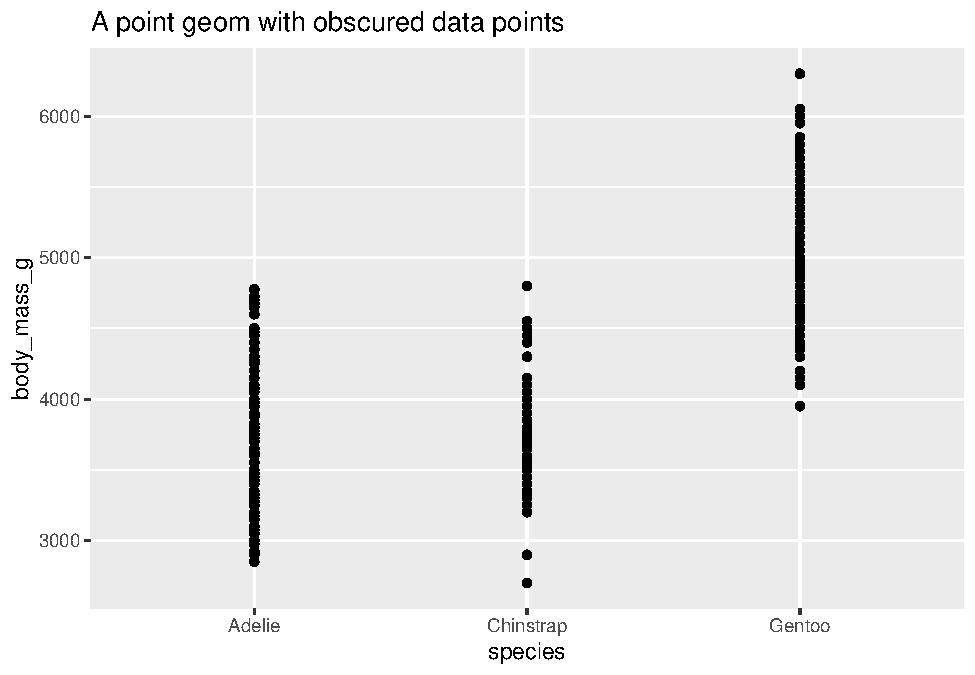
\includegraphics{Grammar-of-Graphics_files/figure-latex/position-1.pdf}

\begin{Shaded}
\begin{Highlighting}[]
\FunctionTok{ggplot}\NormalTok{(}\AttributeTok{data =}\NormalTok{ penguins, }\AttributeTok{mapping =} \FunctionTok{aes}\NormalTok{(}\AttributeTok{x =}\NormalTok{ species, }\AttributeTok{y =}\NormalTok{ body\_mass\_g)) }\SpecialCharTok{+}
  \FunctionTok{geom\_jitter}\NormalTok{() }\SpecialCharTok{+}
  \FunctionTok{ggtitle}\NormalTok{(}\StringTok{"A point geom with jittered data points"}\NormalTok{)}
\end{Highlighting}
\end{Shaded}

\begin{verbatim}
## Warning: Removed 2 rows containing missing values (geom_point).
\end{verbatim}

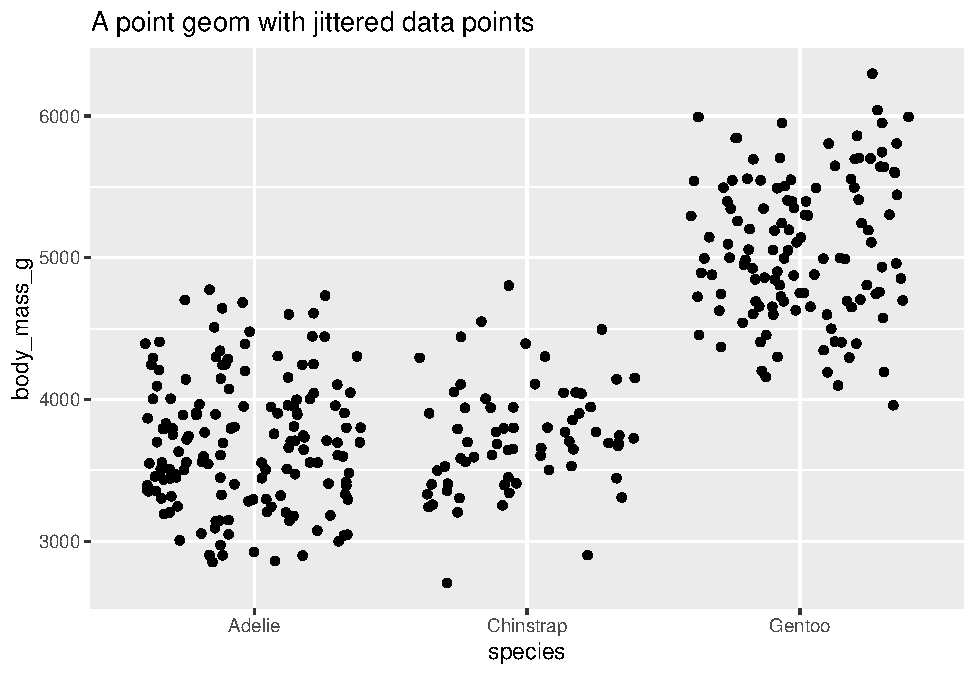
\includegraphics{Grammar-of-Graphics_files/figure-latex/position-2.pdf}

\hypertarget{scale}{%
\subsection{Scale}\label{scale}}

A \textbf{scale} controls how data is mapped to aesthetic attributes, so
we need one scale for every aesthetic property employed in a layer. For
example, this graph defines a scale for color:

\begin{Shaded}
\begin{Highlighting}[]
\FunctionTok{ggplot}\NormalTok{(}\AttributeTok{data =}\NormalTok{ penguins, }\AttributeTok{mapping =} \FunctionTok{aes}\NormalTok{(}\AttributeTok{x =}\NormalTok{ bill\_depth\_mm, }\AttributeTok{y =}\NormalTok{ bill\_length\_mm, }\AttributeTok{color =}\NormalTok{ species)) }\SpecialCharTok{+}
  \FunctionTok{geom\_point}\NormalTok{() }
\end{Highlighting}
\end{Shaded}

\begin{verbatim}
## Warning: Removed 2 rows containing missing values (geom_point).
\end{verbatim}

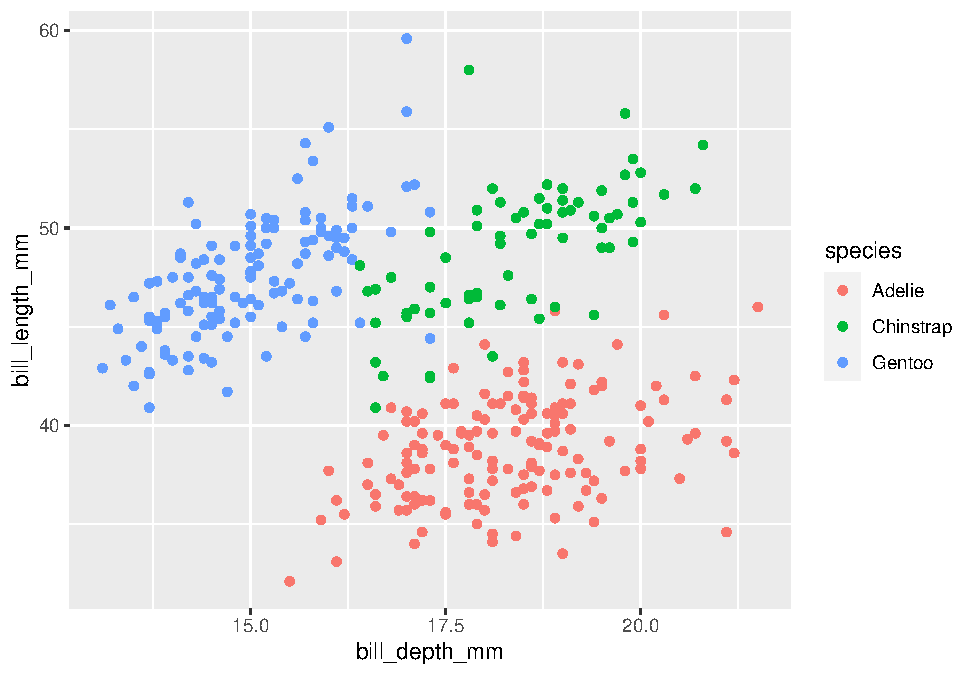
\includegraphics{Grammar-of-Graphics_files/figure-latex/scale_color-1.pdf}

Note that the scale is consistent - every point for a compact car is
drawn in tan, whereas SUVs are drawn in pink. The scale can be changed
to use a different color palette:

\begin{Shaded}
\begin{Highlighting}[]
\FunctionTok{ggplot}\NormalTok{(}\AttributeTok{data =}\NormalTok{ penguins, }\AttributeTok{mapping =} \FunctionTok{aes}\NormalTok{(}\AttributeTok{x =}\NormalTok{ bill\_length\_mm, }\AttributeTok{y =}\NormalTok{ body\_mass\_g, }\AttributeTok{color =}\NormalTok{ species)) }\SpecialCharTok{+}
  \FunctionTok{geom\_point}\NormalTok{() }\SpecialCharTok{+}
  \FunctionTok{scale\_color\_brewer}\NormalTok{(}\AttributeTok{palette =} \StringTok{"Dark2"}\NormalTok{)}
\end{Highlighting}
\end{Shaded}

\begin{verbatim}
## Warning: Removed 2 rows containing missing values (geom_point).
\end{verbatim}

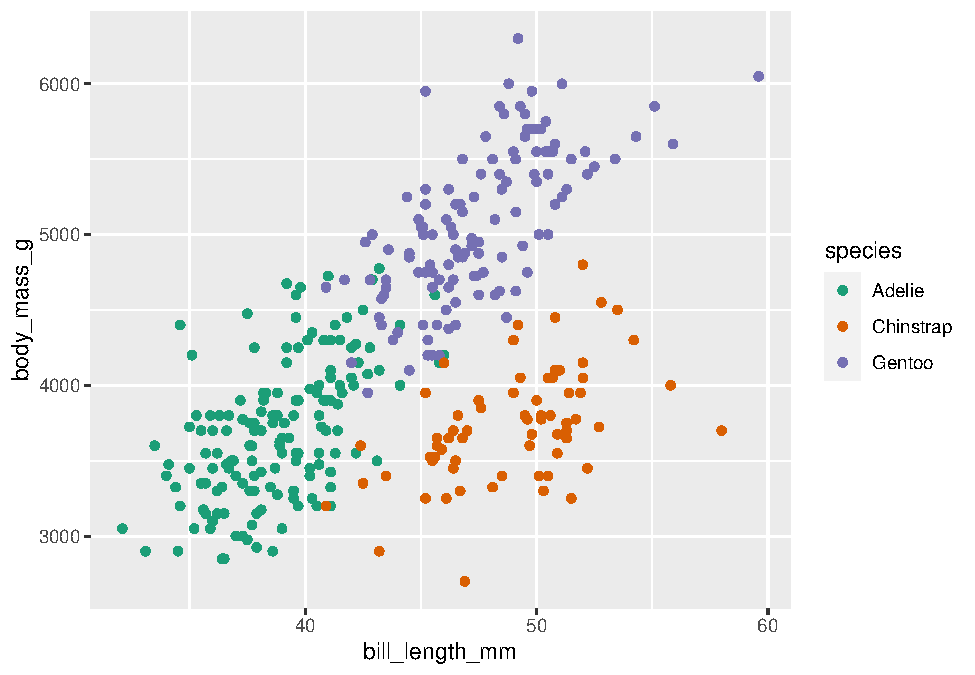
\includegraphics{Grammar-of-Graphics_files/figure-latex/scale_color_palette-1.pdf}

Now we are using a different palette, but the scale is still consistent:
all Adelie penguins utilize the same color, whereas Chinstrap use a new
color \textbf{but each Adelie still uses the same, consistent color}.

\hypertarget{coordinate-system}{%
\subsection{Coordinate system}\label{coordinate-system}}

A \textbf{coordinate system} (\emph{coord}) maps the position of objects
onto the plane of the plot, and controls how the axes and grid lines are
drawn. Plots typically use two coordinates (\(x, y\)), but could use any
number of coordinates. Most plots are drawn using the
\href{https://en.wikipedia.org/wiki/Cartesian_coordinate_system}{\textbf{Cartesian
coordinate system}}:

\begin{Shaded}
\begin{Highlighting}[]
\NormalTok{x1 }\OtherTok{\textless{}{-}} \FunctionTok{c}\NormalTok{(}\DecValTok{1}\NormalTok{, }\DecValTok{10}\NormalTok{)}
\NormalTok{y1 }\OtherTok{\textless{}{-}} \FunctionTok{c}\NormalTok{(}\DecValTok{1}\NormalTok{, }\DecValTok{5}\NormalTok{)}
\NormalTok{p }\OtherTok{\textless{}{-}} \FunctionTok{qplot}\NormalTok{(}\AttributeTok{x =}\NormalTok{ x1, }\AttributeTok{y =}\NormalTok{ y1, }\AttributeTok{geom =} \StringTok{"blank"}\NormalTok{, }\AttributeTok{xlab =} \ConstantTok{NULL}\NormalTok{, }\AttributeTok{ylab =} \ConstantTok{NULL}\NormalTok{) }\SpecialCharTok{+}
  \FunctionTok{theme\_bw}\NormalTok{()}
\NormalTok{p }\SpecialCharTok{+}
  \FunctionTok{ggtitle}\NormalTok{(}\AttributeTok{label =} \StringTok{"Cartesian coordinate system"}\NormalTok{)}
\end{Highlighting}
\end{Shaded}

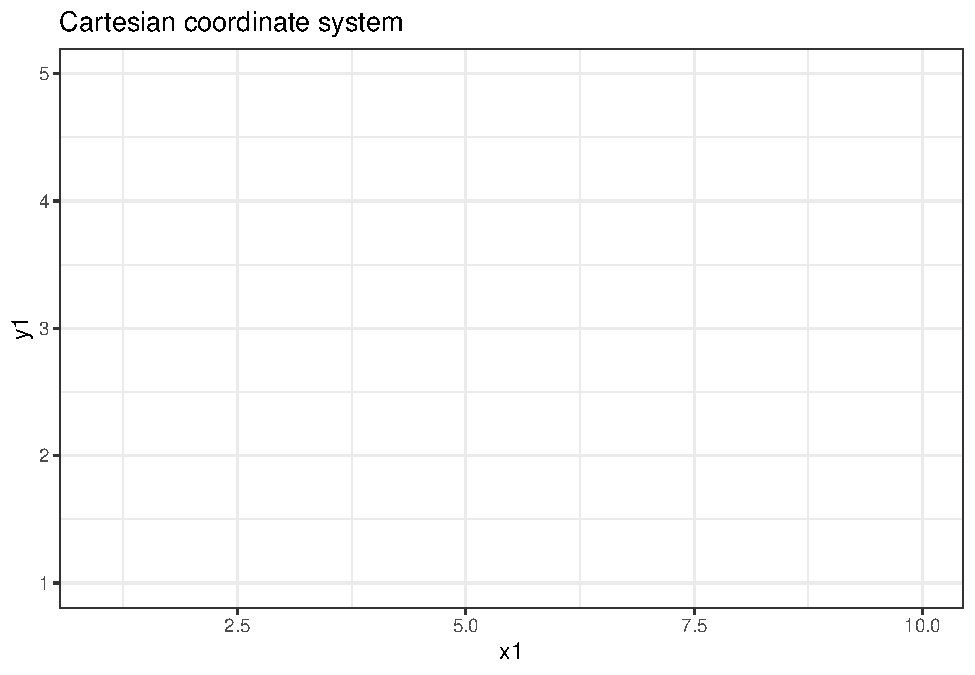
\includegraphics{Grammar-of-Graphics_files/figure-latex/coord_cart-1.pdf}

This system requires a fixed and equal spacing between values on the
axes. That is, the graph draws the same distance between 1 and 2 as it
does between 5 and 6. The graph could be drawn using a
\href{https://en.wikipedia.org/wiki/Semi-log_plot}{\textbf{semi-log
coordinate system}} which logarithmically compresses the distance on an
axis:

\begin{Shaded}
\begin{Highlighting}[]
\NormalTok{p }\SpecialCharTok{+}
  \FunctionTok{coord\_trans}\NormalTok{(}\AttributeTok{y =} \StringTok{"log10"}\NormalTok{) }\SpecialCharTok{+}
  \FunctionTok{ggtitle}\NormalTok{(}\AttributeTok{label =} \StringTok{"Semi{-}log coordinate system"}\NormalTok{)}
\end{Highlighting}
\end{Shaded}

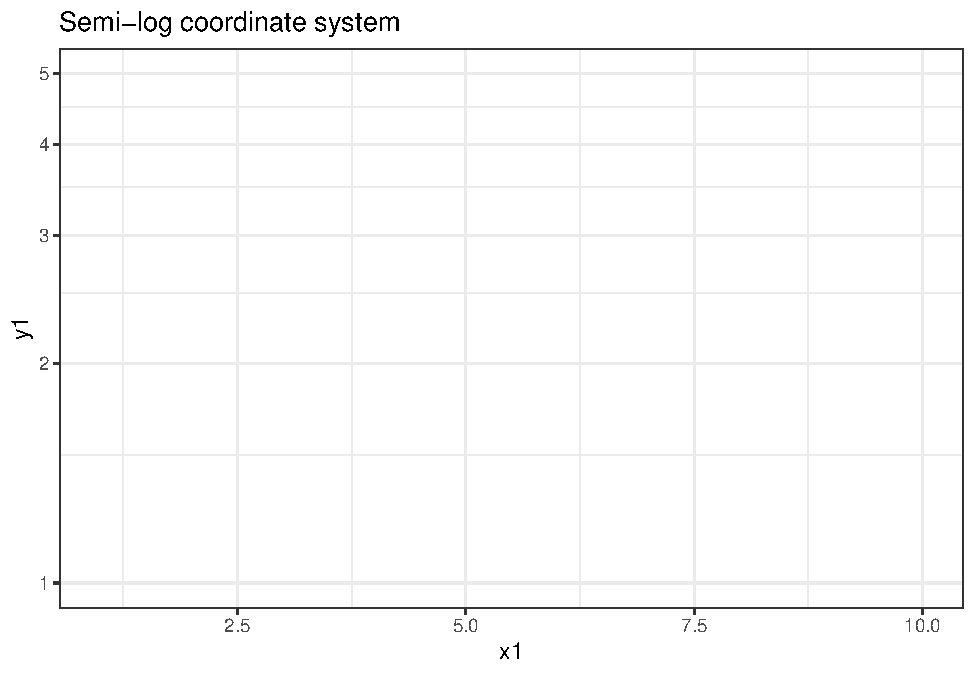
\includegraphics{Grammar-of-Graphics_files/figure-latex/coord_semi_log-1.pdf}

Or could even be drawn using
\href{https://en.wikipedia.org/wiki/Polar_coordinate_system}{\textbf{polar
coordinates}}:

\begin{Shaded}
\begin{Highlighting}[]
\NormalTok{p }\SpecialCharTok{+}
  \FunctionTok{coord\_polar}\NormalTok{() }\SpecialCharTok{+}
  \FunctionTok{ggtitle}\NormalTok{(}\AttributeTok{label =} \StringTok{"Polar coordinate system"}\NormalTok{)}
\end{Highlighting}
\end{Shaded}

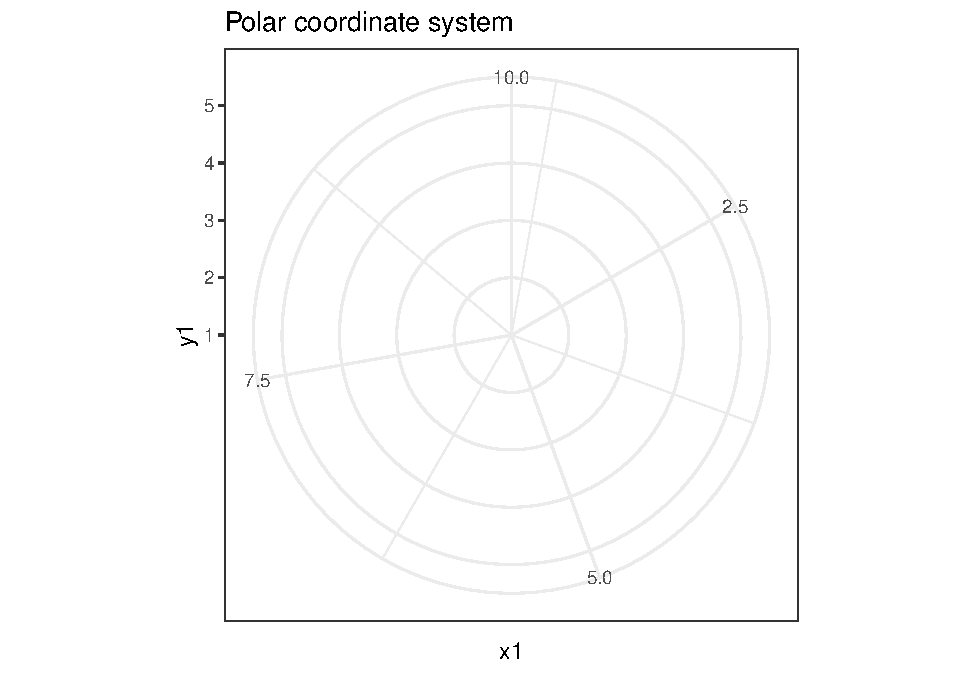
\includegraphics{Grammar-of-Graphics_files/figure-latex/coord_polar-1.pdf}

\hypertarget{faceting}{%
\subsection{Faceting}\label{faceting}}

\textbf{Faceting} can be used to split the data up into subsets of the
entire dataset. This is a powerful tool when investigating whether
patterns are the same or different across conditions, and allows the
subsets to be visualized on the same plot (known as \textbf{conditioned}
or \textbf{trellis} plots). The faceting specification describes which
variables should be used to split up the data, and how they should be
arranged.

\begin{Shaded}
\begin{Highlighting}[]
\FunctionTok{ggplot}\NormalTok{(}\AttributeTok{data =}\NormalTok{ penguins, }\AttributeTok{mapping =} \FunctionTok{aes}\NormalTok{(}\AttributeTok{x =}\NormalTok{ bill\_length\_mm, }\AttributeTok{y =}\NormalTok{ body\_mass\_g)) }\SpecialCharTok{+}
  \FunctionTok{geom\_point}\NormalTok{() }\SpecialCharTok{+}
  \FunctionTok{facet\_wrap}\NormalTok{(}\SpecialCharTok{\textasciitilde{}}\NormalTok{species)}
\end{Highlighting}
\end{Shaded}

\begin{verbatim}
## Warning: Removed 2 rows containing missing values (geom_point).
\end{verbatim}

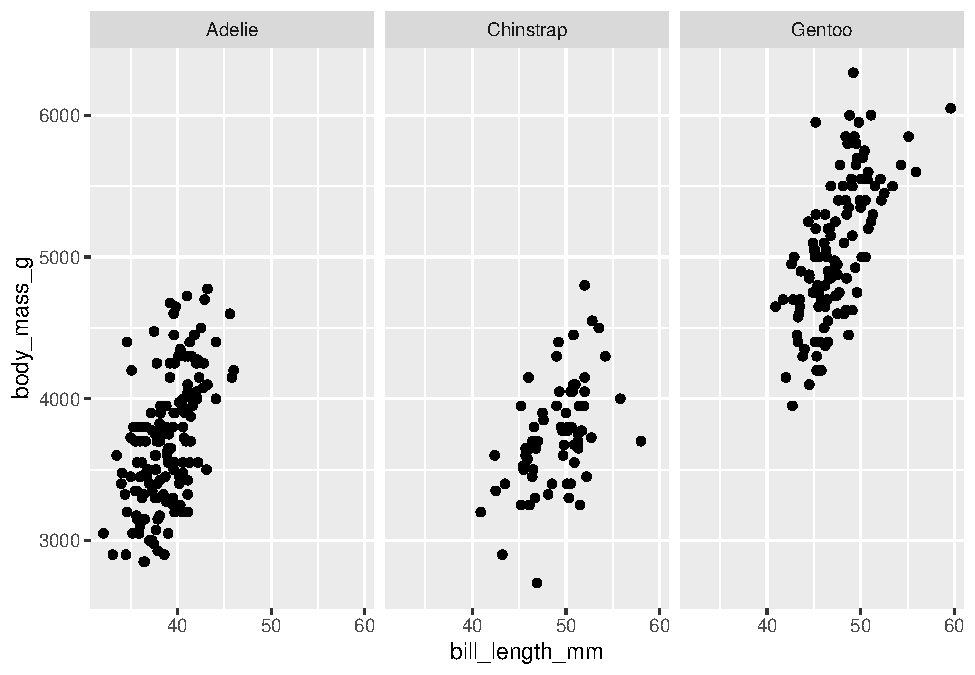
\includegraphics{Grammar-of-Graphics_files/figure-latex/facet-1-1.pdf}

\begin{Shaded}
\begin{Highlighting}[]
\CommentTok{\# ggplot(data = penguins, mapping = aes(x = bill\_length\_mm, y = body\_mass\_g, color = sex)) +}
\CommentTok{\#   geom\_point(aes(x = sex)) +}
\CommentTok{\#   facet\_grid(species\textasciitilde{}island)}

\CommentTok{\# Ria\textquotesingle{}s explanation: This code did not work becasue....}
\end{Highlighting}
\end{Shaded}

\hypertarget{defaults}{%
\subsection{Defaults}\label{defaults}}

Rather than explicitly declaring each component of a layered graphic
(which will use more code and introduces opportunities for errors), we
can establish intelligent defaults for specific geoms and scales. For
instance, whenever we want to use a bar geom, we can default to using a
stat that counts the number of observations in each group of our
variable in the \(x\) position.

Consider the following scenario: you wish to generate a scatterplot
visualizing the relationship between penguins' bill\_length and their
body\_mass. With no defaults, the code to generate this graph is:

\begin{Shaded}
\begin{Highlighting}[]
\FunctionTok{ggplot}\NormalTok{() }\SpecialCharTok{+}
  \FunctionTok{layer}\NormalTok{(}
    \AttributeTok{data =}\NormalTok{ penguins, }\AttributeTok{mapping =} \FunctionTok{aes}\NormalTok{(}\AttributeTok{x =}\NormalTok{ bill\_length\_mm, }\AttributeTok{y =}\NormalTok{ body\_mass\_g),}
    \AttributeTok{geom =} \StringTok{"point"}\NormalTok{, }\AttributeTok{stat =} \StringTok{"identity"}\NormalTok{, }\AttributeTok{position =} \StringTok{"identity"}
\NormalTok{  ) }\SpecialCharTok{+}
  \FunctionTok{scale\_x\_continuous}\NormalTok{() }\SpecialCharTok{+}
  \FunctionTok{scale\_y\_continuous}\NormalTok{() }\SpecialCharTok{+}
  \FunctionTok{coord\_cartesian}\NormalTok{()}
\end{Highlighting}
\end{Shaded}

\begin{verbatim}
## Warning: Removed 2 rows containing missing values (geom_point).
\end{verbatim}

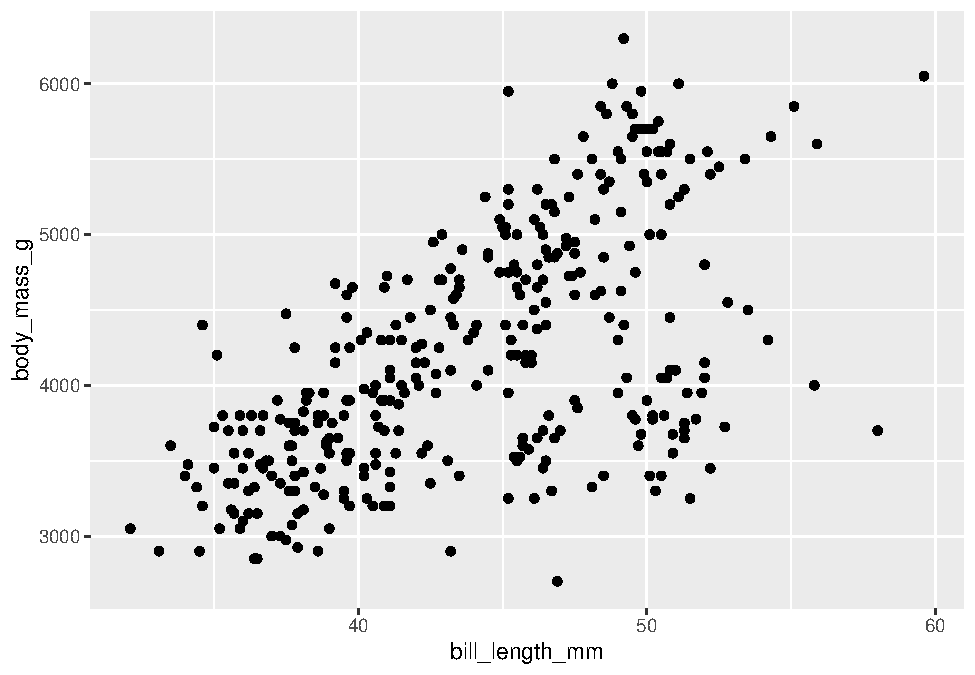
\includegraphics{Grammar-of-Graphics_files/figure-latex/default-1.pdf}

The above code:

\begin{itemize}
\item
  Creates a new plot object (\texttt{ggplot})
\item
  Adds a layer (\texttt{layer})

  \begin{itemize}
  \tightlist
  \item
    Specifies the data (\texttt{penguins})
  \item
    Maps engine bill length to the \(x\) position and body mass to the
    \(y\) position (\texttt{mapping})
  \item
    Uses the point geometric transformation (\texttt{geom\ =\ "point"})
  \item
    Implements an identity transformation and position
    (\texttt{stat\ =\ "identity"} and \texttt{position\ =\ "identity"})
  \end{itemize}
\item
  Establishes two continuous position scales
  (\texttt{scale\_x\_continuous} and \texttt{scale\_y\_continuous})
\item
  Declares a cartesian coordinate system (\texttt{coord\_cartesian})
\end{itemize}

How can we simplify this using intelligent defaults?

\begin{enumerate}
\def\labelenumi{\arabic{enumi}.}
\item
  We only need to specify one geom and stat, since each geom has a
  default stat.
\item
  Cartesian coordinate systems are most commonly used, so it should be
  the default.
\item
  Default scales can be added based on the aesthetic and type of
  variables.

  \begin{itemize}
  \tightlist
  \item
    Continuous values are transformed with a linear scaling.
  \item
    Discrete values are mapped to integers.
  \item
    Scales for aesthetics such as color, fill, and size can also be
    intelligently defaulted.
  \end{itemize}
\end{enumerate}

Using these defaults, we can rewrite the above code as:

\begin{Shaded}
\begin{Highlighting}[]
\FunctionTok{ggplot}\NormalTok{() }\SpecialCharTok{+}
  \FunctionTok{geom\_point}\NormalTok{(}\AttributeTok{data =}\NormalTok{ penguins, }\AttributeTok{mapping =} \FunctionTok{aes}\NormalTok{(}\AttributeTok{x =}\NormalTok{ bill\_length\_mm, }\AttributeTok{y =}\NormalTok{ body\_mass\_g))}
\end{Highlighting}
\end{Shaded}

\begin{verbatim}
## Warning: Removed 2 rows containing missing values (geom_point).
\end{verbatim}

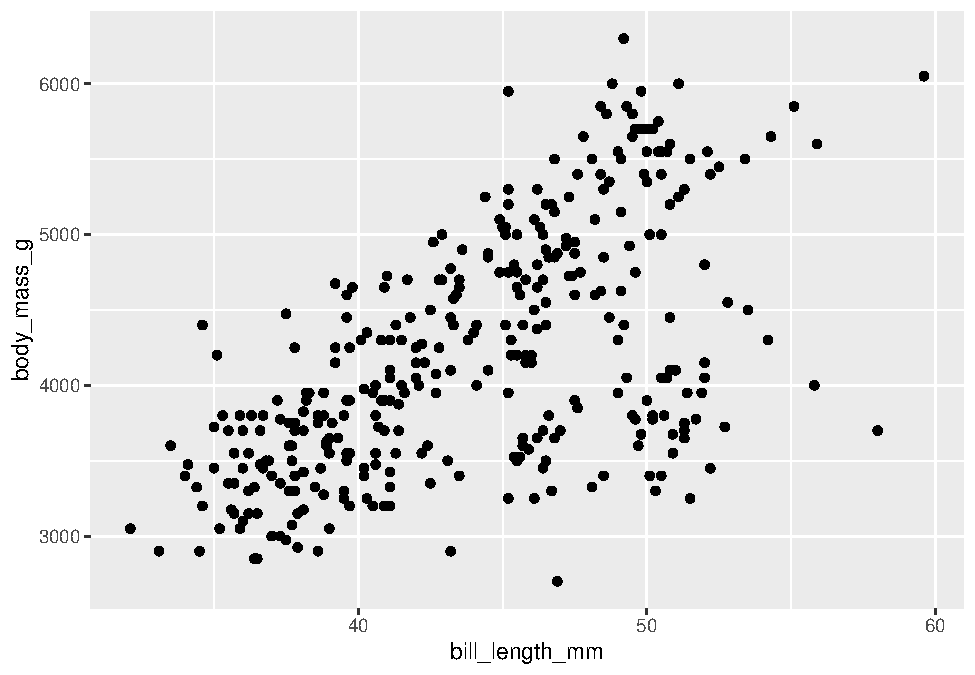
\includegraphics{Grammar-of-Graphics_files/figure-latex/default2-1.pdf}

This generates the exact same plot, but uses fewer lines of code.
Because multiple layers can use the same components (data, mapping,
etc.), we can also specify that information in the \texttt{ggplot()}
function rather than in the \texttt{layer()} function:

\begin{Shaded}
\begin{Highlighting}[]
\FunctionTok{ggplot}\NormalTok{(}\AttributeTok{data =}\NormalTok{ penguins, }\AttributeTok{mapping =} \FunctionTok{aes}\NormalTok{(}\AttributeTok{x =}\NormalTok{ bill\_length\_mm, }\AttributeTok{y =}\NormalTok{ body\_mass\_g)) }\SpecialCharTok{+}
  \FunctionTok{geom\_point}\NormalTok{()}
\end{Highlighting}
\end{Shaded}

\begin{verbatim}
## Warning: Removed 2 rows containing missing values (geom_point).
\end{verbatim}

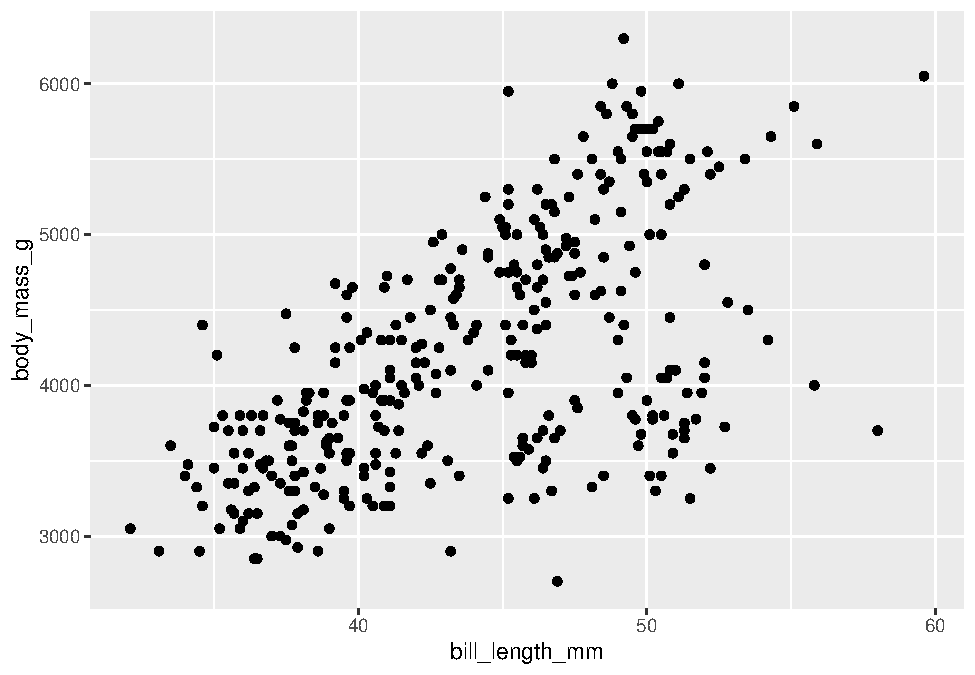
\includegraphics{Grammar-of-Graphics_files/figure-latex/default3-1.pdf}

And as we will learn, function arguments in R use specific ordering, so
we can omit the explicit call to \texttt{data} and \texttt{mapping}:

\begin{Shaded}
\begin{Highlighting}[]
\FunctionTok{ggplot}\NormalTok{(penguins, }\FunctionTok{aes}\NormalTok{(bill\_length\_mm, body\_mass\_g)) }\SpecialCharTok{+}
  \FunctionTok{geom\_point}\NormalTok{()}
\end{Highlighting}
\end{Shaded}

\begin{verbatim}
## Warning: Removed 2 rows containing missing values (geom_point).
\end{verbatim}

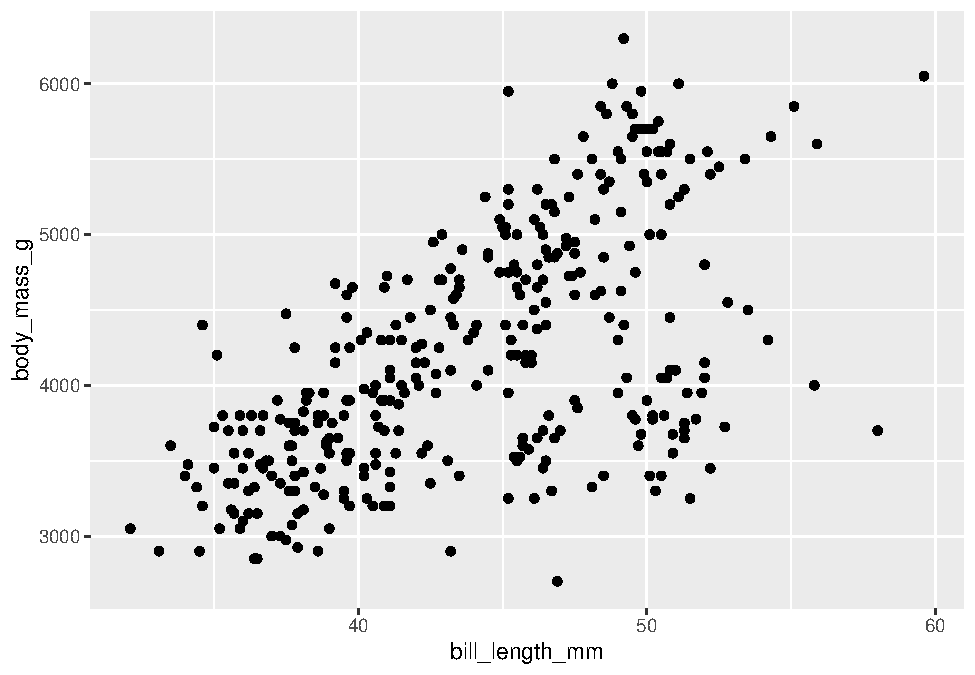
\includegraphics{Grammar-of-Graphics_files/figure-latex/default4-1.pdf}

\end{document}
